\addcontentsline{toc}{section}{Converting FAME to AWI Workspace (Airbus)}
\section*{Converting FAME to AWI Workspace (Airbus)}
This section provides a discussion on: 
\begin{itemize}
\item The process through which the AWI framework is able to read and convert the FAME files into the MATLAB workspace
\item The assumptions made by the framework regarding which files are needed and where they are expected to exist in the available folder structure.
\end{itemize}
\addcontentsline{toc}{subsection}{Assumptions about the FAME folder structure}
\subsection*{Assumptions about the FAME folder structure}

An example of the type of folder structure expected by the AWI framework is presented in figure \ref{fig:FAMEFolderStructure}. It is important to note in most cases the framework will give the user the ability to locate the required files if it is not able to find them. File and folder requirements are discussed below.

\begin{enumerate}
	\item \textbf{Main entry point} - The main entry point to the FAME files is the \textbf{*.fm4} file. This is highlighted in blue in figure \ref{fig:FAMEFolderStructure}. The framework assumes that one of the parent folders of the fm4 file is labelled \textbf{`06$\_$weights'}. In the case where such a parent folder does not exist, the framework's assumed path structure will fail and will consequently request the user to find the required files as they are needed by the framework. Therefore, the assumed path structure is not critical but it is preferable. Currently, the \textbf{*.fm4} is expected to exist in the \textbf{$\_\_$mirror} folder as illustrated in figure \ref{fig:FAMEFolderStructure}. If the framework realises that $\_\_$mirror folder is not the immediate parent folder of the *.fm4 file, then it asks the user to select the main FAME output folder which is generally labelled \textbf{*-pv8}. A check is performed to ensure that the `$\_\_$mirror', `1$\_$structure', and 'export' folders exist in the newly selected FAME folder.
	\item \textbf{*tux$\_$xml file} - The `tux$\_$xml' file is expected to exist in a folder called \textbf{`01$\_$geometry'} at a similar level to where the `06$\_$weights' is found. If the framework fails to find this file it will ask the user to locate the file for it. This folder is used to extract geometries of the aircraft which may be missing from the fm4 file.
	\item \textbf{FAME results} - The fame results (deformations, internal loads, aerodynamic loads etc.) are expected in the \textbf{`*.m1-1-pv8/export/fmwpp01/flexible'} folder. If the results are not found then the import process will step out without looking for the following files:
	\begin{enumerate}	
		\item \textbf{Load Case file} - Information about the load cases are currently retrieved from the \textbf{`loadcase$\_$info.txt'} file, as it contains more information than is available in the fm4 file. It is assumed that this file is located in \textbf{`*.m1-1-pv8/1$\_$structure/1$\_$10$\_$wing/13$\_$fame-w/flexible'}. If the file is not found, the framework will ask the user to locate it.
		\item \textbf{Nastran files} - A nastran file which is generated by the FAME sizing process and contains GRID, PBAR, CBAR and MAT1 entries is currently used by the framework to discretise the wing in to a series of finite beam elements. The framework is only interested in the following file \textbf{`*.m1-1pv8/1$\_$structure/1$\_$10$\_$wing/13$\_$fame-w/flexible/deformations /model$\_$nastran$\_\_$ldcase0001.dat'}. The rest of the nastran files, containing the point loads associated to each load case are used to extract the loads and not the beam properties.
		\item \textbf{Wing mass files} - The framework assumes that the wing mass file is contained in the folder \textbf{`$\_\_$mon/wbd2/massdist/flexible'}. It expects files of the form `*.205'. In the case where it finds both an unsorted and sorted file (\textbf{massdist$\_$items.205} and \textbf{`massdist$\_$items $\_\_$sorted.205'}) the framework will prioritise the sorted file and extract both the primary and secondary masses.
		\item \textbf{Fuel mass files} - The fuel mass files are expected to exist in \textbf{`$\_\_$mon/wbd2/massdist/ flexible'}. Given that the naming of the fuel files are arbitrary and subject to the Airbus user, the framework currently performs a search criteria within that folder for any files with the name \textbf{`right*'}. If the framework is unable to find any files of that type, then it will ask the user to find the files. It is not critical to select all of the fuel files but preferable if all are selected, as the fuel mass closest to that specified in the loadcase will be assigned to the beam model later on in the aeroelastic analysis. 
	\end{enumerate}
\end{enumerate}
\begin{figure}[h!]
\centering
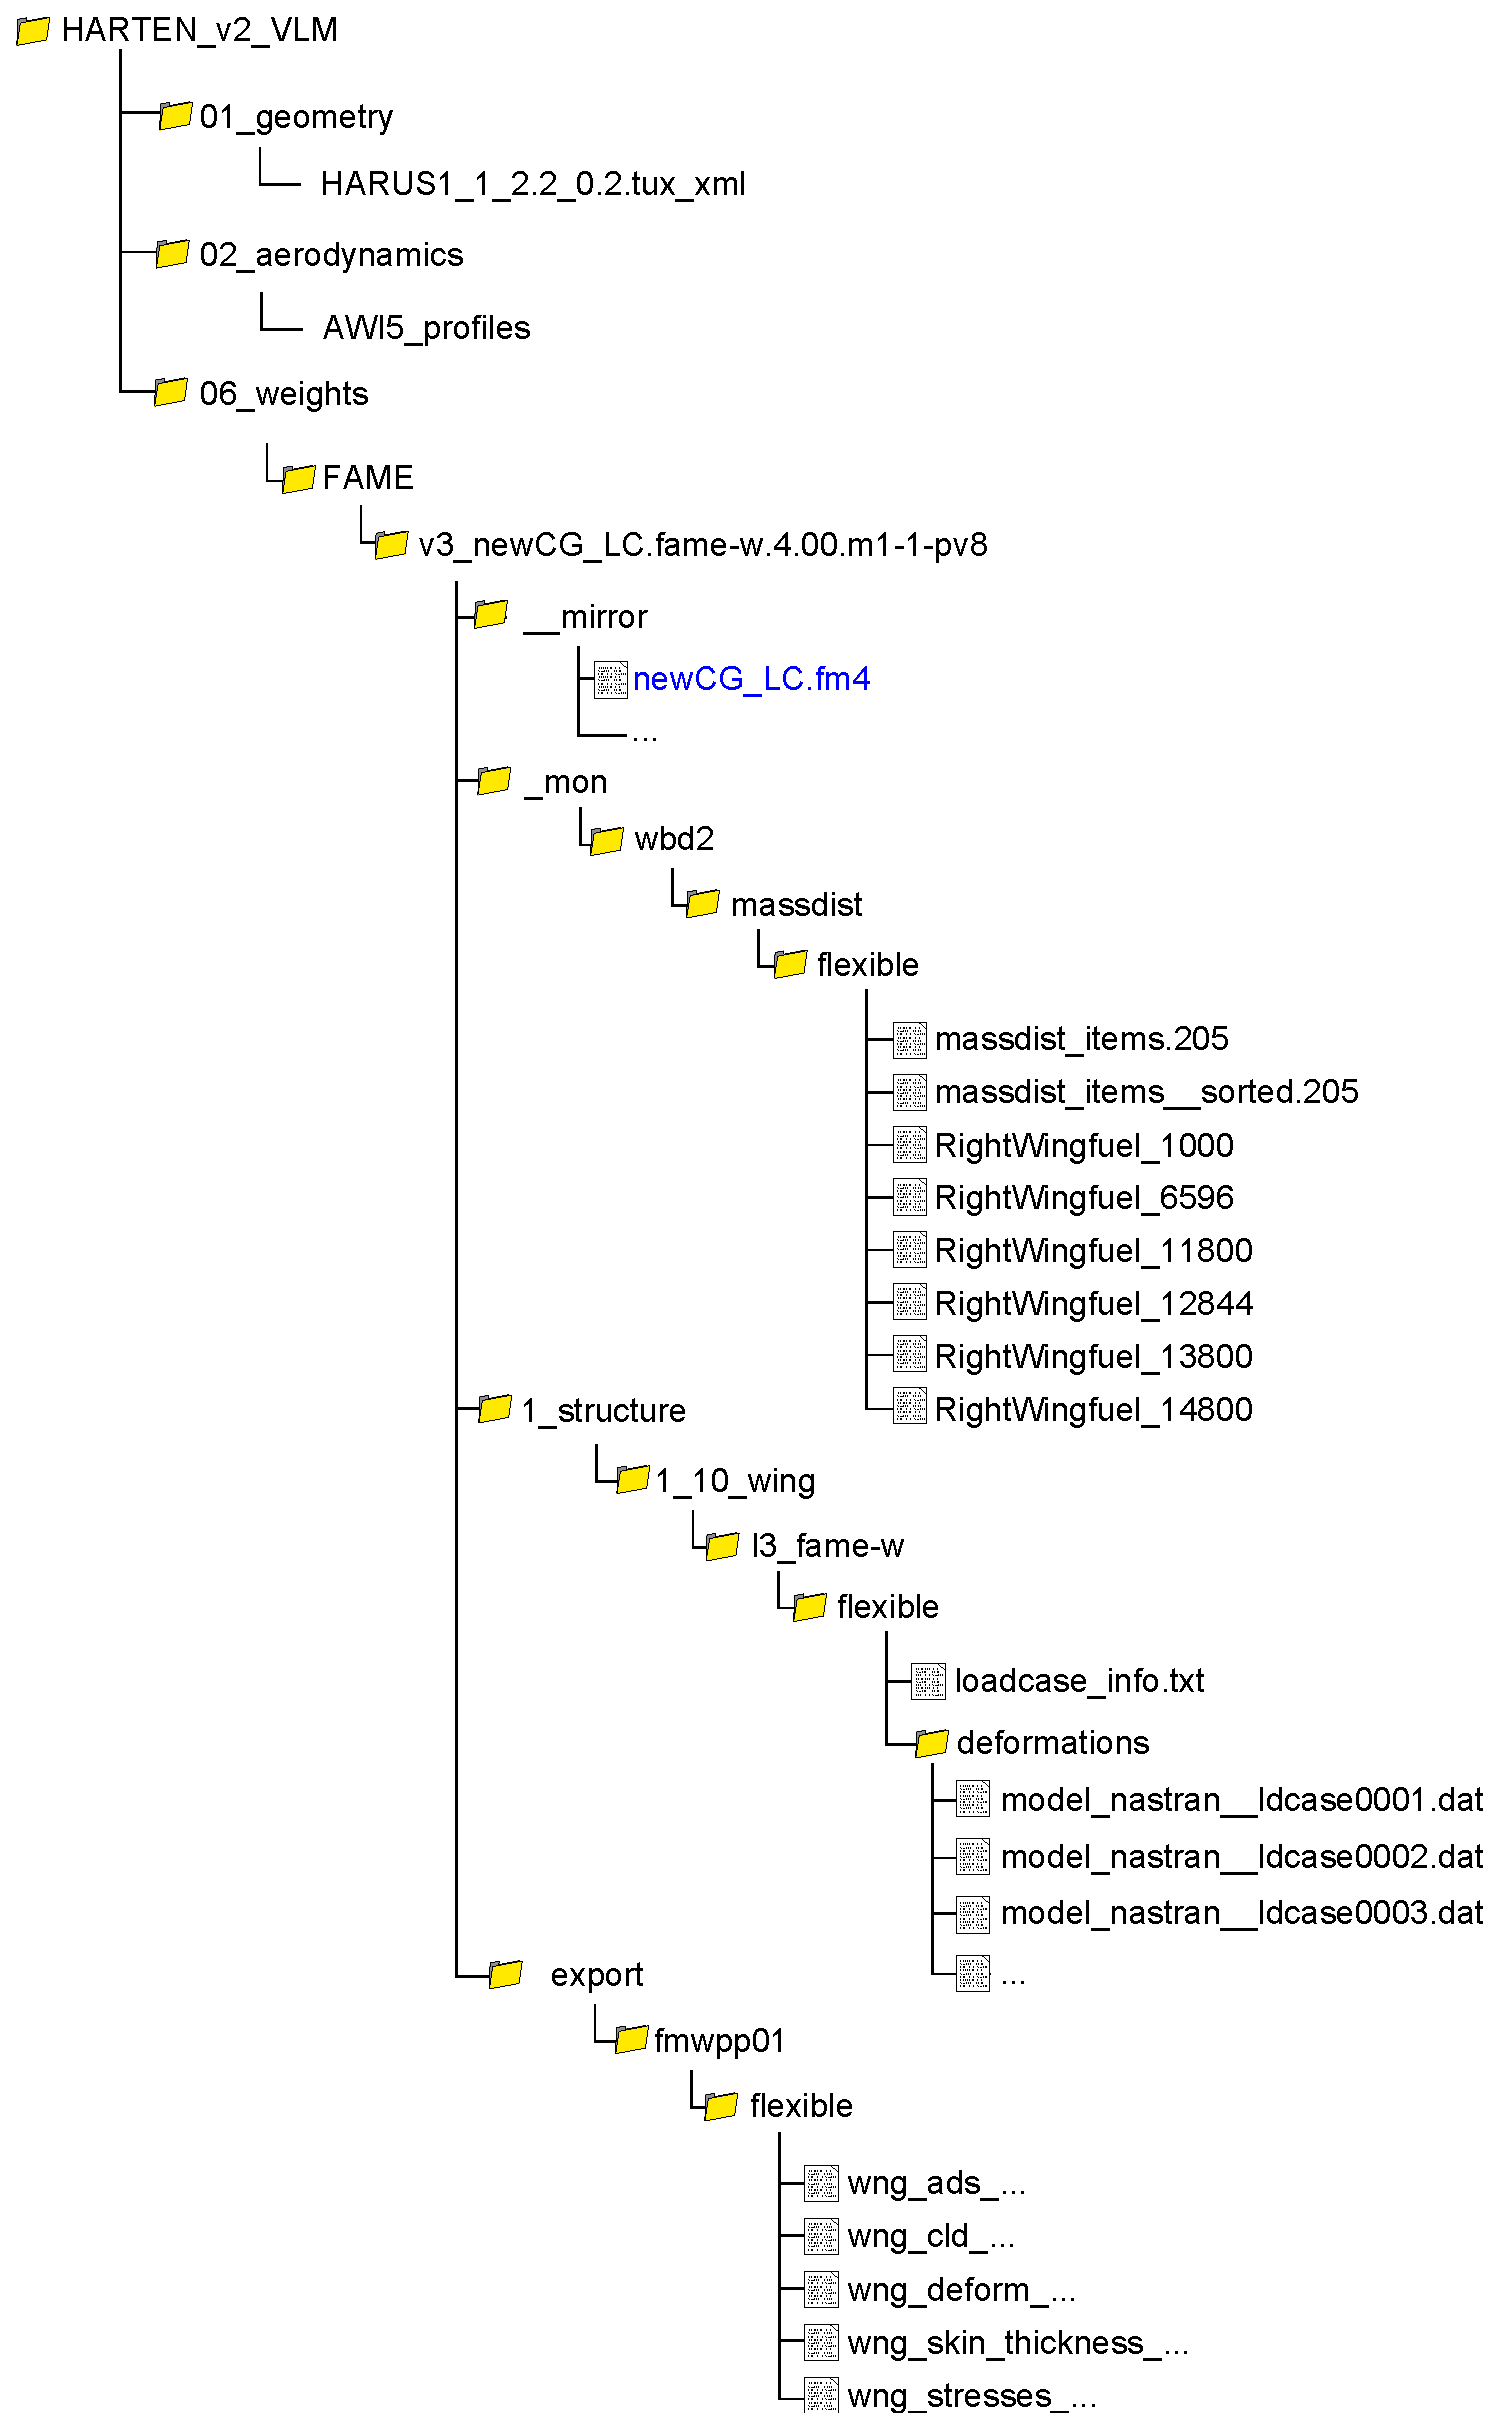
\includegraphics[width=0.7\textwidth]{FAMEFolderStructure}
\caption{FAME Folder Structure}\label{fig:FAMEFolderStructure}
\end{figure}

\addcontentsline{toc}{subsection}{An explanation on the FAME import procedures}
\subsection*{An explanation on the FAME import procedures}

\begin{enumerate}
\item \textbf{Read *fm4 file} - The first step in the FAME import process is to read and parse the input file into the MATLAB workspace. The underlying function ``getFameInput'' grabs all of the information found in this single file, and creates a structure array that preserves the structure in the file. \textbf{N.B.} It is important to note that the current version ignores `INCLUDE' entries in the file and therefore, pertinent information, which will be outlined further on, must be explicitly written into the .fm4 file. 

\item \textbf{Read *tux$\_$xml file} - The `tux$\_$xml' file is also used by the FAME file reader. Since FAME-W is a wing sizing tool, empennage geometries are usually omitted from the .fm4 file. The AWI framework circumvents this by extracting all of the information found in the tux file and isolating the `vtp' and `htp' entries to create the empennage geometries. An outline of the aerodynamic surfaces is created and later used to generate a finite element model. Control surfaces are added to the `vtp' and `htp'. Engine and fuselage geometries are also used by the AWI framework if they exist in the `tux$\_$xml' file.

\item \textbf{Read FAME results} - The FAME results are then extracted and stored internally.

\item \textbf{Read FAME Nastran File} - A nastran finite element model is automatically generated by the FAME sizing process and passed into the AWI framework. The beam elements in this file belong to the wing and contain stiffness properties which correspond to the 3-dimensional properties of the internal wing sections obtained through the FAME sizing. Figure \ref{fig:FAMENastranModel} illustrates the original beam model extracted from FAME.

\begin{figure}[h!]
\centering
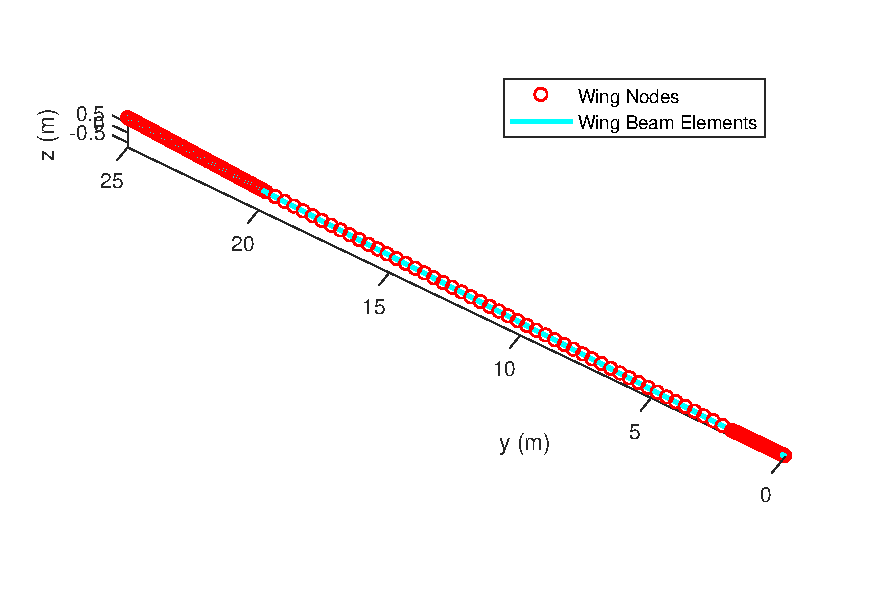
\includegraphics[width = 0.7\textwidth]{FAMENastranModel}
\caption{FAME Nastran finite element model}\label{fig:FAMENastranModel}
\end{figure}

\begin{figure}[h!]
\centering
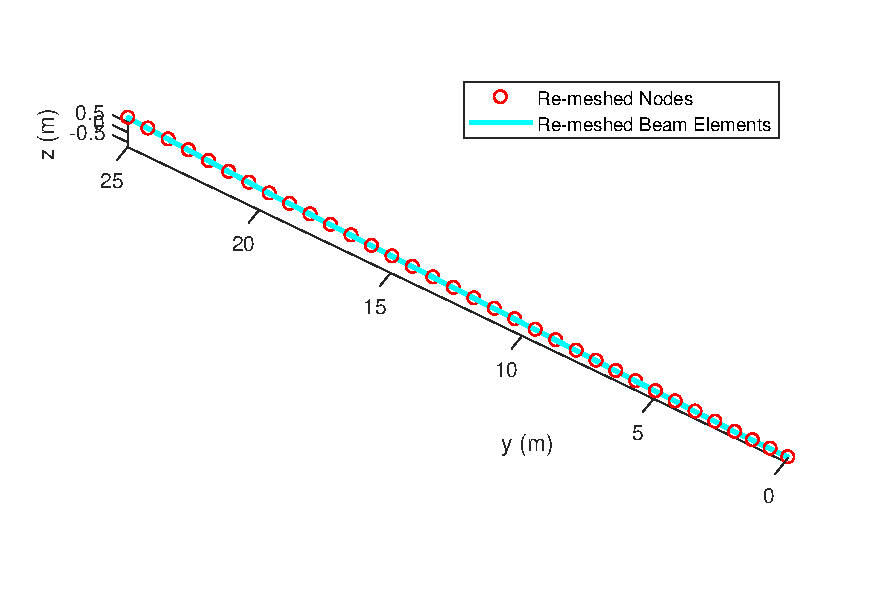
\includegraphics[width = 0.7\textwidth]{FAMENastranModelRe-meshed}
\caption{Reduced FAME finite element model}\label{fig:FAMENastranModelReduced}
\end{figure}

It is often the case that the FAME wing beam model is made up of a large number of beam elements ($>$150). In order to improve the simulation run time this beam model can be re-meshed. Currently, the re-meshing takes place during the import process and cannot be altered after the fact. However, the ability to arbitrarily discretise the beam model from within the framework will be added in a future version. An example of a beam model which has been reduced to 32 beam elements is shown in figure \ref{fig:FAMENastranModelReduced}. A comparison between the stiffness properties of the original and the reduced beam model is presented in figure \ref{fig:OriginalvsReducedStiffness}.

\begin{figure}[h!]
\centering
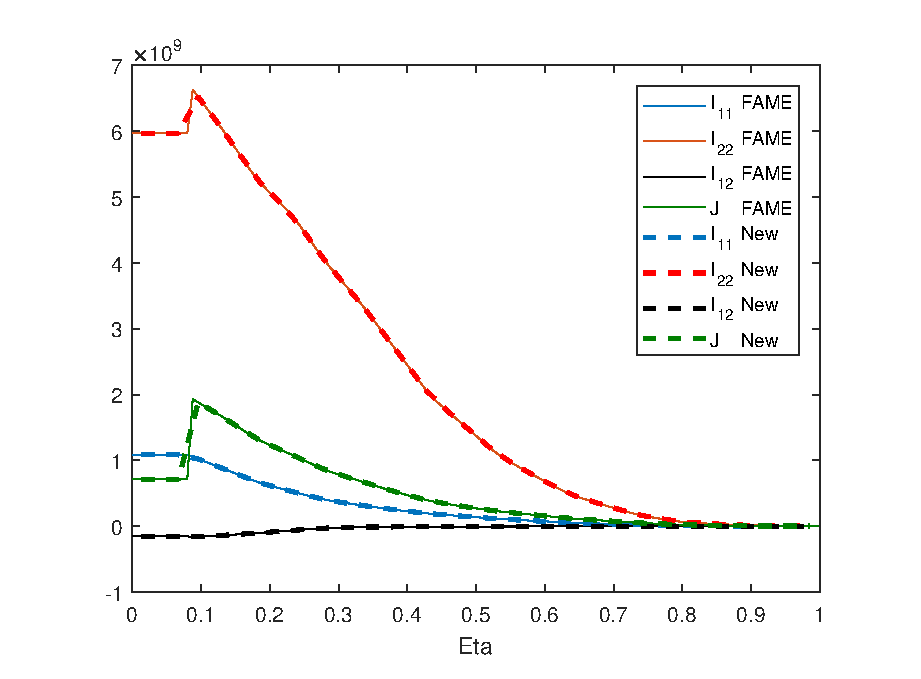
\includegraphics[width = 0.7\textwidth]{StiffnessComparison}
\caption{A comparison of the sectional properties of the FAME model, before and after model reduction}\label{fig:OriginalvsReducedStiffness}
\end{figure}

\item \textbf{Get Wing Masses} - The wing masses are extracted from the .205 file in the FAME folder. The process consists of retrieving the mass, centre of gravity and mass moment of inertia of each point mass and consolidating them onto a single lumped mass per node along the wing. Figure \ref{fig:OriginalFAMEMasses} illustrates the original masses taken from FAME and figure \ref{fig:ReducedFAMEMasses} shows the aggregation of these masses according to the reduced finite element model.

\begin{figure}[h!]
\centering
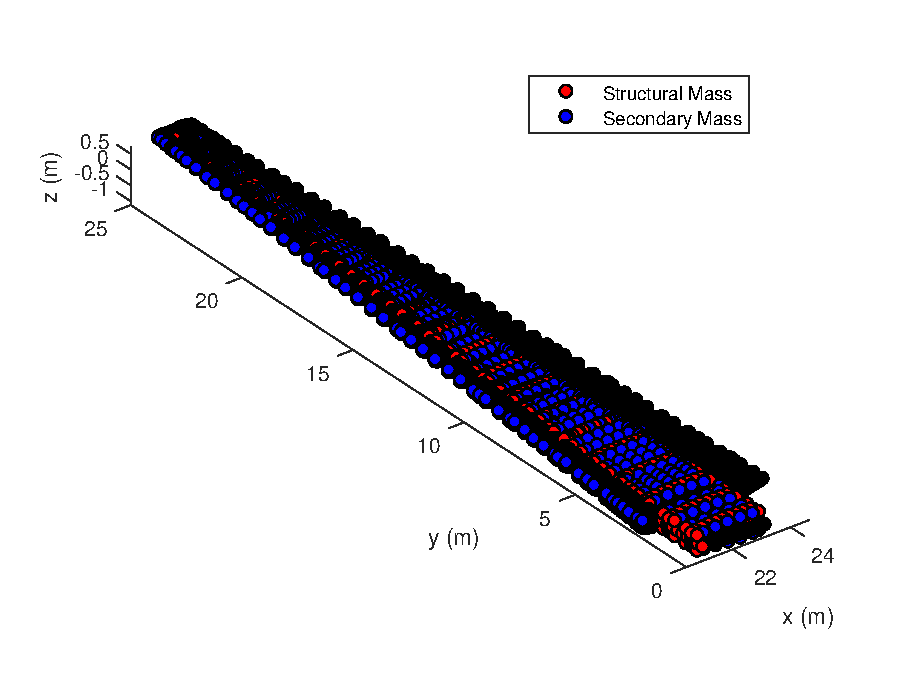
\includegraphics[width = 0.7\textwidth]{OriginalFAMEMasses}
\caption{FAME lumped masses representing primary and secondary masses}\label{fig:OriginalFAMEMasses}
\end{figure}

\begin{figure}[h!]
\centering
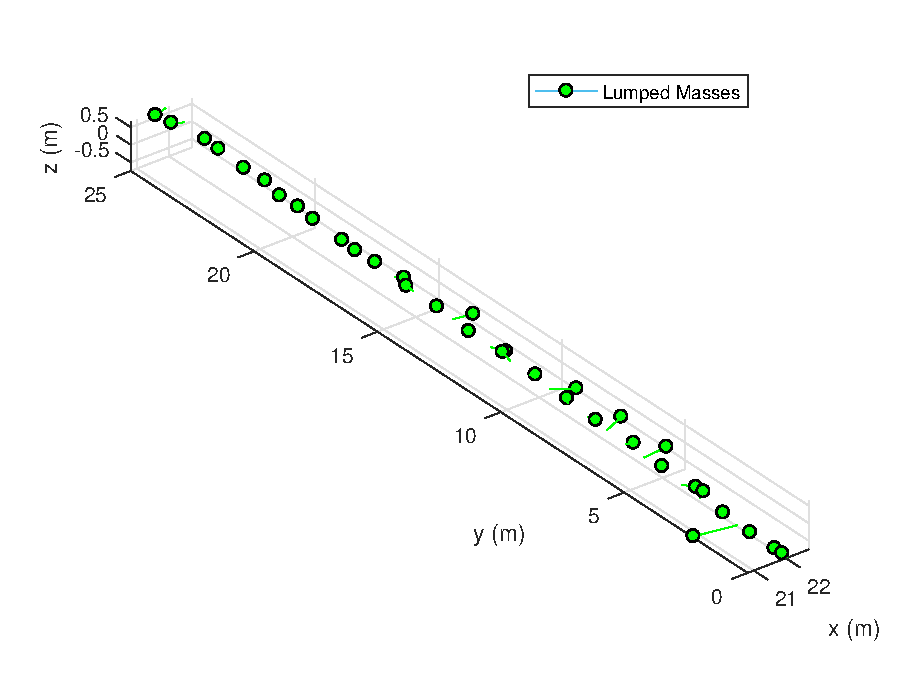
\includegraphics[width = 0.7\textwidth]{ReducedFAMEMasses}
\caption{Reduced FAME lumped masses for the primary and secondary mass}\label{fig:ReducedFAMEMasses}
\end{figure}

\item \textbf{Get Fuel Masses} - The fuel mass distribution is obtained from aformentioned user created files which contain point masses for each fuel configuration. The number of point masses is reduced in a similar manner to the wing mass. The fuel is stored separately and treated as a special mass which is associated to a particular load case. 

\item \textbf{Define additional masses} - In addition to the wing masses and the fuel masses the import process must assign mass to the rest of the aircraft. The empennage consists of rigid beam elements coupled to lumped masses to represent its mass. Given that the mass of the empennage is not specified anywhere in the FAME sizing process, an estimate is made. 

\begin{itemize}
\item \textbf{Engine} - If the engine is wing-mounted then the position and mass is directly transferred to the finite element model. If it is rear-mounted and defined in the tux$\_$xml file, then the engine mass is estimated and placed accordingly. 
\item \textbf{HTP} - The HTP mass is estimated at 0.9\% of the MTOW specified in the fm4 file.
\item \textbf{VTP} - The VTP mass is estimated at 1.4\% of the MTOW specified in the fm4 file.
\item \textbf{Fuselage} - The fuselage mass is estimated by ensuring that the lumped masses in the finite element model add up to the OEW. If the OEW is not specified anywhere in the FAME input files then it is estimated at 25\% of the MTOW specified in the fm4 file.
\end{itemize}

\item \textbf{Define aerodynamic surfaces} - Figure \ref{fig:FAMEAerodynamicSurface} illustrates the aerodynamic surfaces generated by the import process. The discretisation of the spanwise aerodynamic panels are chosen to match the beam elements, therefore, a one-to-one correspondance exists.  

\begin{figure}[h!]
\centering
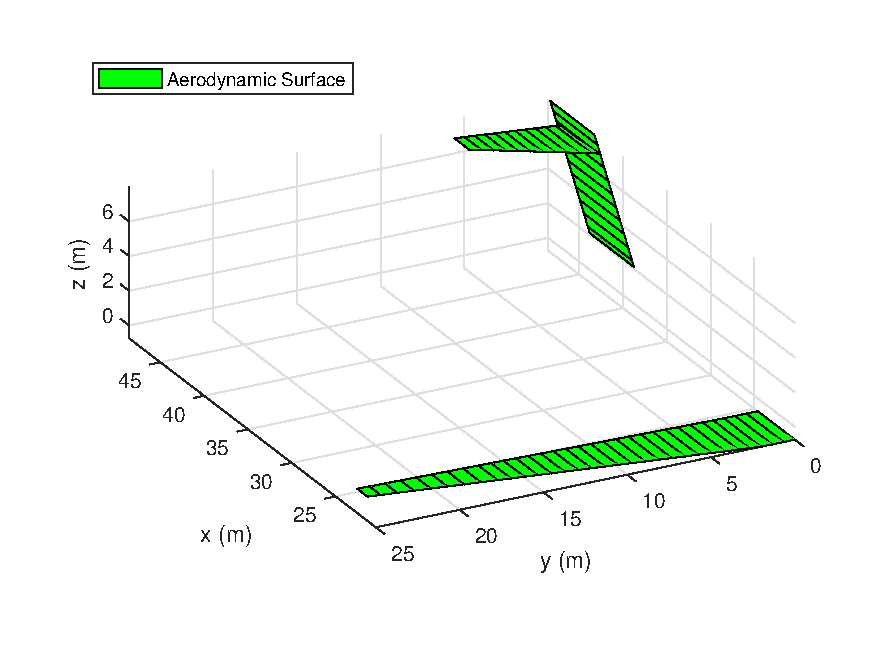
\includegraphics[width = 0.7\textwidth]{FAMEAerodynamicSurface}
\caption{Reduced FAME lumped masses for the primary and secondary mass}\label{fig:FAMEAerodynamicSurface}
\end{figure}

\item \textbf{Define aerodynamic nodes} - Figure \ref{fig:FAMEAerodynamicNodes} illustrates the aerodynamic nodes generated by the import process, which are then used to create interploation sets for the aerodynamic surfaces and the structural grids. 

\begin{figure}[h!]
\centering
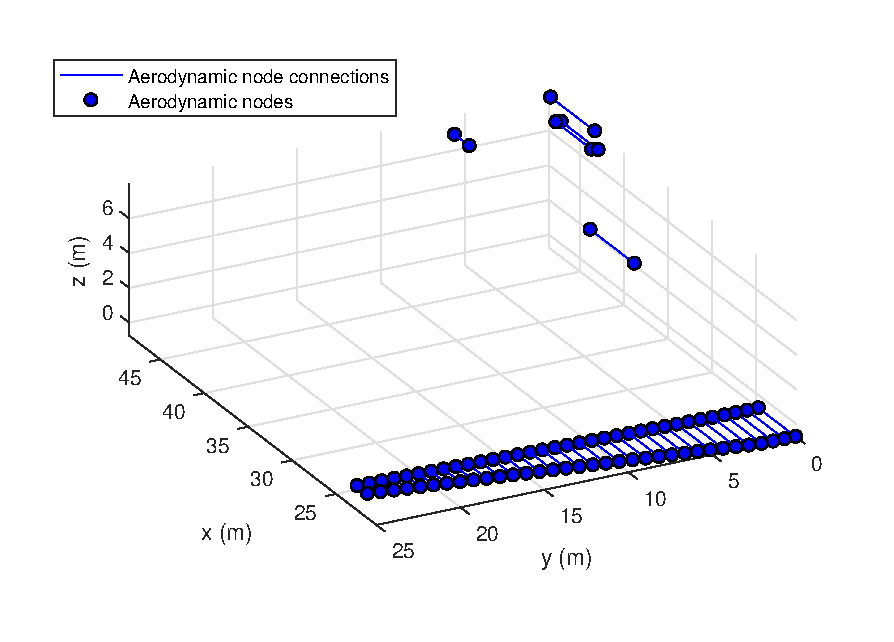
\includegraphics[width = 0.7\textwidth]{FAMEAerodynamicNodes}
\caption{Aerodynamic nodes and their corresponding connections, used for splining between aerodynamics surfaces and structural grid nodes}\label{fig:FAMEAerodynamicNodes}
\end{figure}

\item \textbf{Reflect the model} - Figure \ref{fig:ReflectedModel} illustrates the reflected aircraft model and figure \ref{fig:FAMEModelFramework} presents the users view of the imported model within the AWI GUI.

\begin{figure}[h!]
\centering
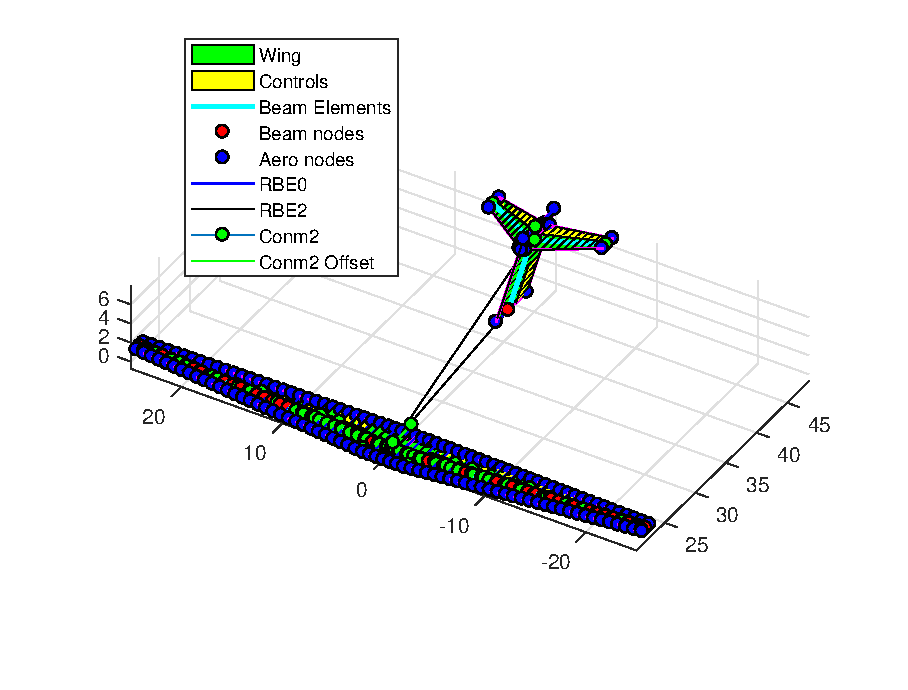
\includegraphics[width = 0.85\textwidth]{ReflectedModel}
\caption{Complete aeroelastic model of the full FAME aircraft}\label{fig:ReflectedModel}
\end{figure}

\begin{figure}[h!]
\centering
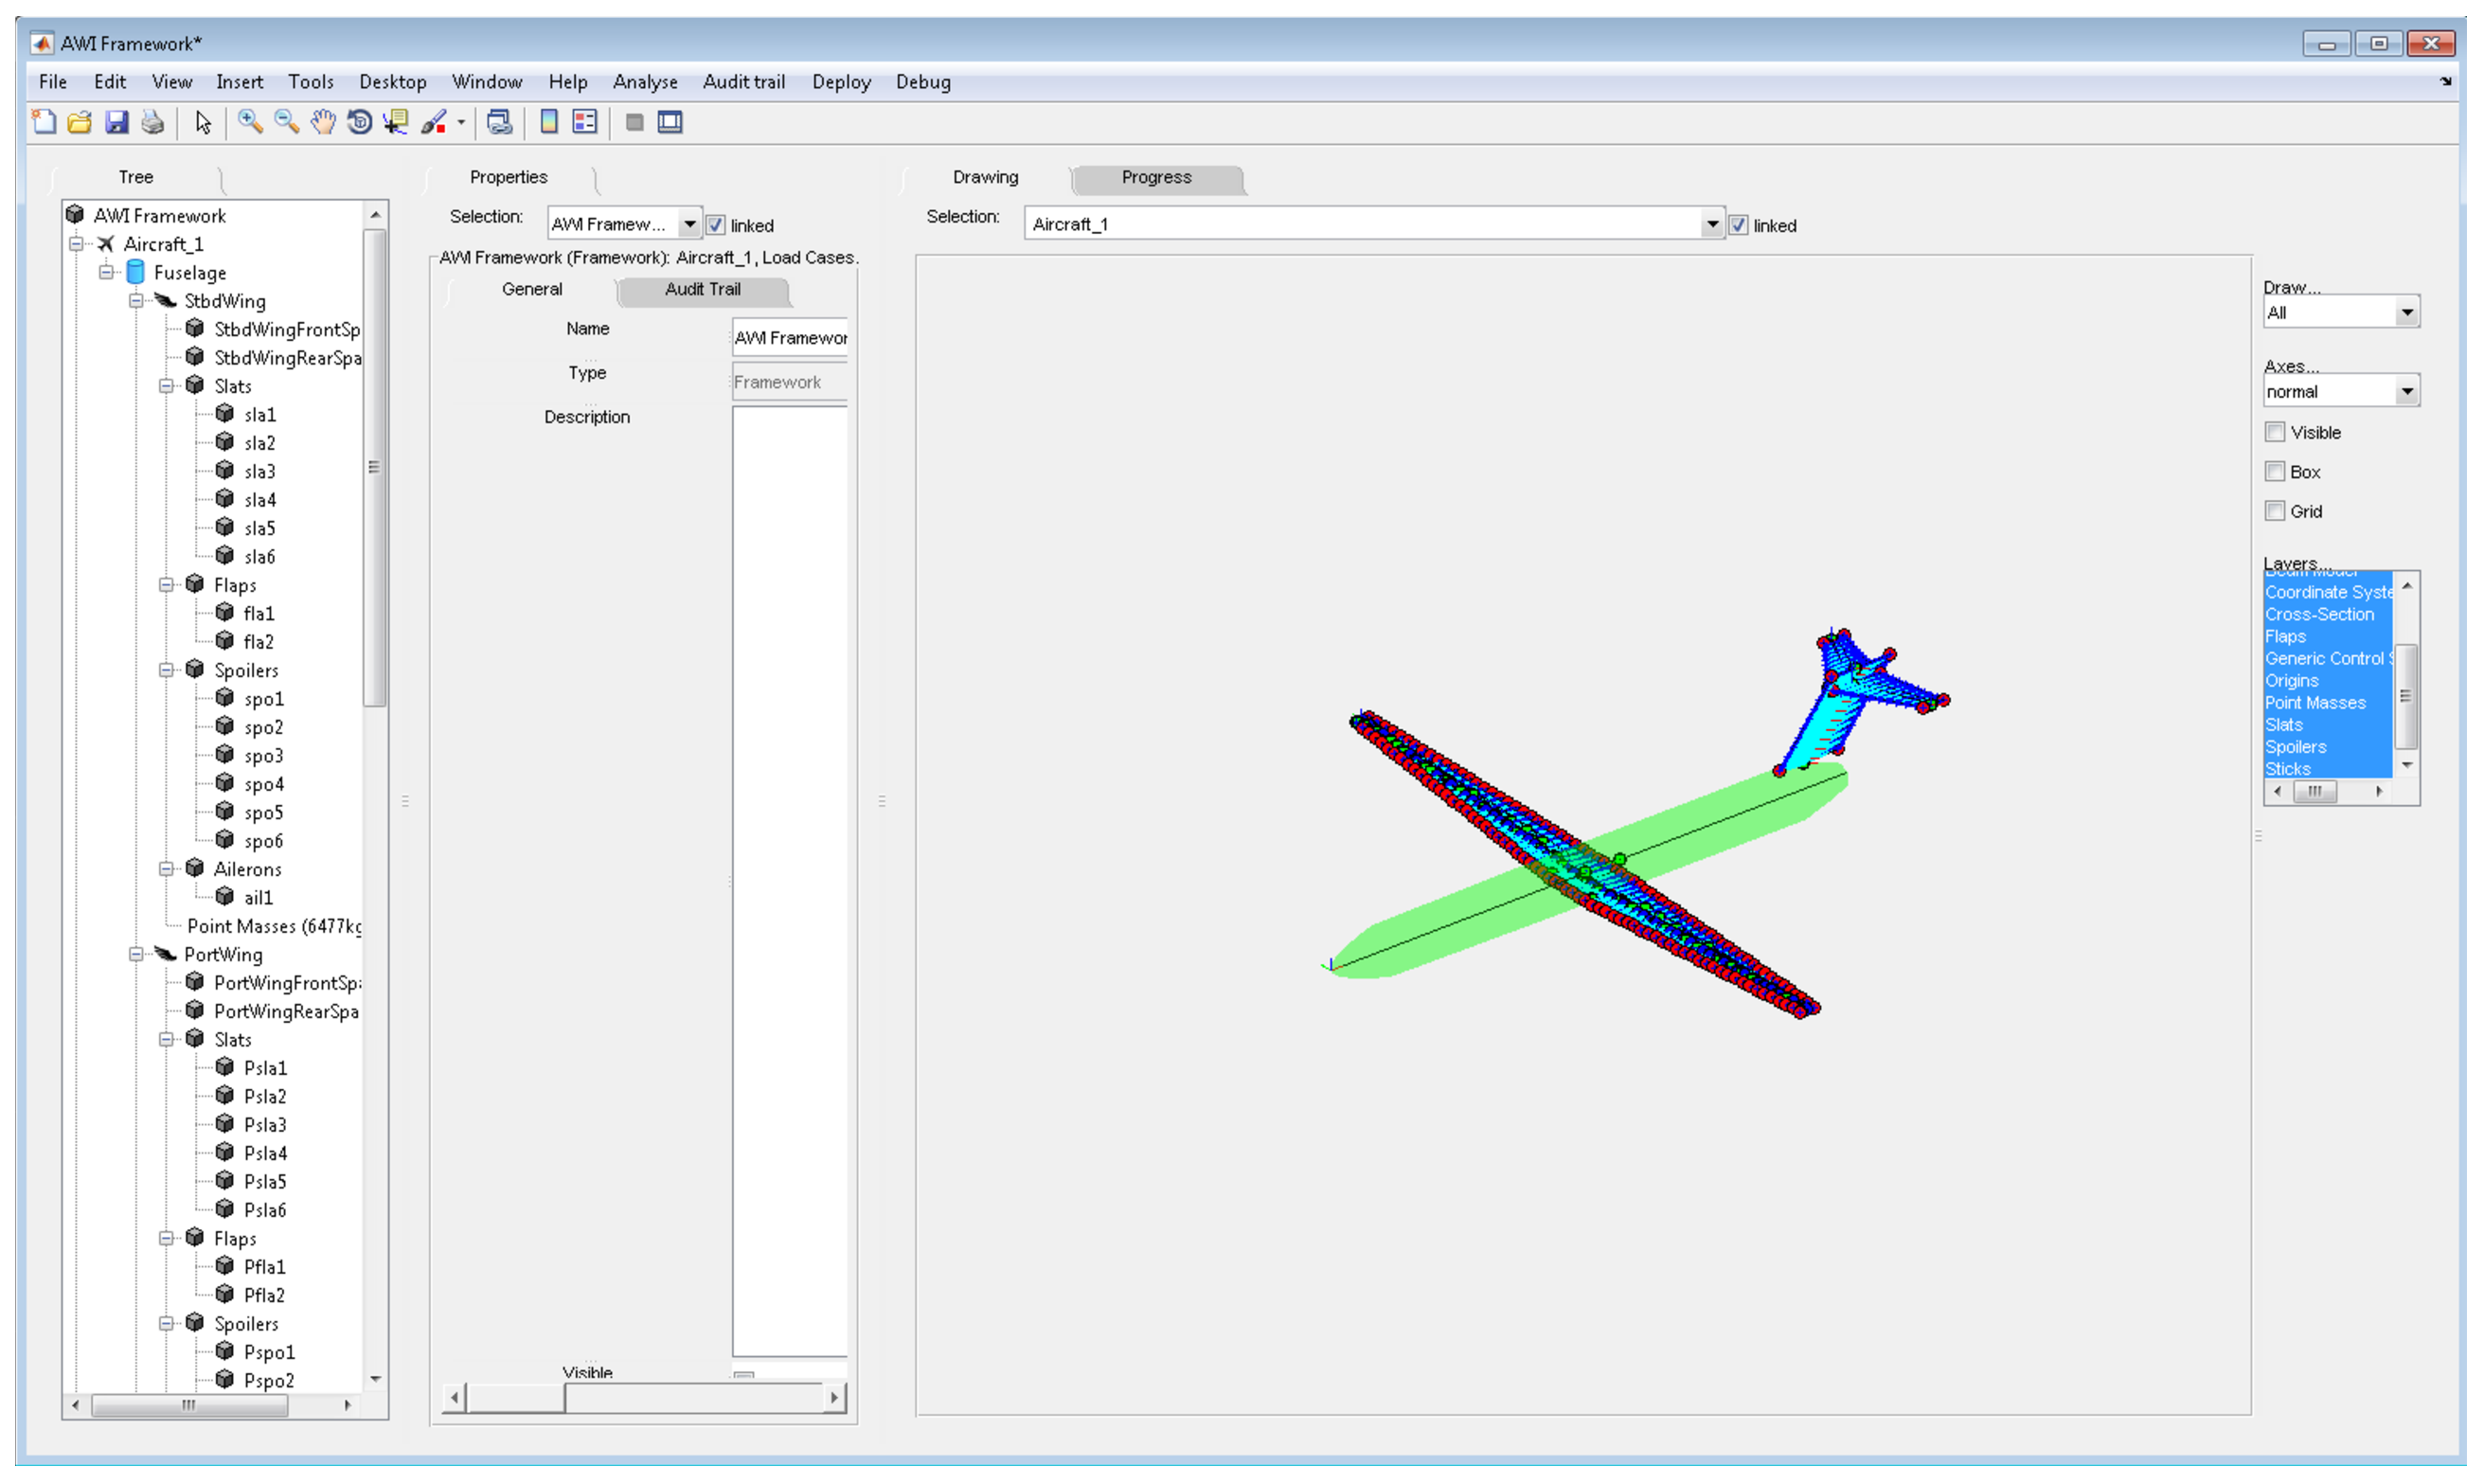
\includegraphics[width = 0.85\textwidth]{FAMEModelFramework}
\caption{Graphical representation of the FAME aircraft/beam model through the AWI GUI}\label{fig:FAMEModelFramework}
\end{figure}

\end{enumerate}
